This the first ever bbZZ analysis performed at CERN with the real data uses the standard set of the CMS
reconstructed physics objects. We describe reconstruction of
electrons, muons, jets and b jets, and MET separately below:



\subsection{Electrons\label{sec:electrons}}
The Gaussian Sum Filter algorithm (GSF
Electrons)~\cite{Khachatryan:2015hwa} is used to reconstruct
electrons. GSF helps to estimate track parameters. The procedure starts as follows: a mixture of Gaussian distributions (normally about 4-6 components) \cite{GSF} is used to estimate the energy loss in each layer of the tracker. The energy loss is modelled by the Bethe-Heitler formula. Two most important track properties are then computed: a weighted mean or the most frequent value (mode). The first estimate is unbiased while the latter one has a smaller width. In practice, mostly one works with the mode. Gaussian mixtures are determined minimising either the absolute difference between the CDFs of the model and of the Gaussian mixture, or the Kullback-Leibner distance, which is a logarithm of the ratio of the pdfs of the model with respect to the mixture. Finally, the tracks are extrapolated further to the ECAL The measurement selects electrons, which pass the following selection: leading electron $\pt>25\GeV$ and subleading electron $\pt>15\GeV$, $|\eta|<2.5$, 
%$d_{xy}<0.05\cm$, $d_z<0.2\cm$ and 
an isolation cut of 0.06, for which the cone
of $0.3$ is used to compute the $\rho$-subtracted PF
isolation. Lepton isolation is calculated as a scalar sum of
the transverse momentum $(p_{T})$ of all the charged and
neutral hadrons as well as photons around the lepton
(excluding the cone) normalised to the $p_{T}$ of the lepton
itself. 
%POG recommended MVA ID WP Loose is further applied to the set of selected electrons.
%The cut on isolation in the measurement for electrons is $0.06$.

        
        %%To emulate the conditions of the HLT trigger, a set of offline cuts is applied further.

%% \texttt{pt>15 \& (}\\
%% \texttt{(abs(superCluster().eta)<1.4442 \& full5x5\_sigmaIetaIeta<0.012 \& }\\
%% \texttt{hcalOverEcal<0.09 \&}\\
%% \texttt{(ecalPFClusterIso/pt)<0.4 \& (hcalPFClusterIso/pt)<0.25 \&}\\
%% \texttt{(dr03TkSumPt/pt)<0.18 \& abs(deltaEtaSuperClusterTrackAtVtx)<0.0095 \&}\\
%% \texttt{abs(deltaPhiSuperClusterTrackAtVtx)<0.065) || }\\
%% \texttt{(abs(superCluster().eta)>1.5660 \& full5x5\_sigmaIetaIeta<0.033 \&}\\
%% \texttt{hcalOverEcal<0.09 \&}\\
%% \texttt{(ecalPFClusterIso/pt)<0.45 \& (hcalPFClusterIso/pt)<0.28 \&}\\
%% \texttt{(dr03TkSumPt/pt)<0.18)}\\
%% \texttt{).}

        On top of the selection defined above, a specific CMS Particle Object Group (POG) recommended working point (WP) is applied, which is a discriminant based on the a multivariate analysis (MVA) for classification of signal/background electrons. The WP consists of nearly 20 variables utilising the information from the impact point, tracks, and the ECAL: $\chi^2 variables$ of the track and the quality of its estimate, $\delta \eta$, $\delta \phi$, energy of the 3 by 3 cluster, ECAL energy over momentum, etc. For this analysis we use the loose working point (another name can be WP90), as described in ~\cite{vhbbAN}. ID and ISO, as well as the HLT SFs are applied.
%        \small{\texttt{https://twiki.cern.ch/twiki/bin/viewauth/CMS/ \\MultivariateElectronIdentificationRun2}}
%\normalsize



\subsection{Muons\label{sec:muons}}
        In this analysis we are using global muons reconstructed using the information from the tracker and muon system \cite{CMS-PAS-MUO-10-002,Chatrchyan:2012xi}. During the offline reconstruction, muons chambers segments are used as seeds for the "standalone muon" reconstruction. The seed is a position, a direction, and an initial momentum of the muon candidate. This serves as an input to the track fitting procedure utilising muon system information. The resulting object after executing this technique is what is called a standalone muon. Then, for each standalone muon the algorithm searches for the tracks reconstructed in the inner tracking system (tracker tracks) that would match the muon. Then for each standalone muon - tracker track pair the Kalman filter based fit \cite{Lenzi:2013xpa} is performed. The result is a collection of muons which are referred to as global muons. In this analysis the kinematic and isolation selection of global muons is the following:
        
leading muon $\pt>20\GeV$ and subleading muon $\pt>15\GeV$, $|\eta|<2.4$,
%re is a loose preselection of $\pt>5\GeV$, $|\eta|<2.4$, $d_{xy}<0.5\cm$, $d_z<1.0\cm$, as well as 
a relative
isolation cut of 0.15, with the cone of $0.4$ used to compute $\Delta\beta$-subtracted PF isolation.
Finally, a tighter selection - muon POG recommended WP Loose is applied~\cite{CMS-PAS-MUO-10-002,MuonsRun2}. WP consists of track quality information: $\chi^2$ of various fits, number of good hits in the tracker, number of layer missing the expected hit, impact parameter variables, matching variables (e.g., a segment in the muon station matched to the tracker track extrapolation), compatibility variables (e.g., a muon segment compatibility). ID, ISO, HLT and tracker SFs are applied.
%The offline cut on isolation for muons is $0.15$.
%% Loose muon:
%% \begin{itemize}
%%   \item  Particle-Flow Muon:\\
%% \texttt{isPFMuon()}
%%   \item  is Global or Tracker Muon:\\
%% \texttt{isGlobalMuon() || isTrackerMuon()}
%%  \end{itemize}

\subsection{Jets\label{sec:jets}}
    Particle flow (PF) algorithm is used to reconstruct jets \cite{CMS-PAS-PFT-09-001,CMS-PAS-PFT-10-001}, with the help of the  $\text{anti}-k_T$ clustering algorithm having a distance parameter of $R=0.4$~\cite{Cacciari:2005hq,Cacciari:2008gp}. Jets are collimated bunches of 	stable hadrons originating from quarks and gluons after fragmentation and hadronization. Therefore, jet finding procedure is a back-propagation that starts with the detected objects and following the rules of the quantum mechanics for fragmentation and hadronization targets to identify the initial partons. \text{anti}-k_T$ is a sequential clustering algorithm that first defines the notion of the distance between the two particles in the collection of particles of the event, and also a distance between the particle and the beam axis. Then sequentially iterating over the particles collection it computes the smallest distances, if the smallest one is between the particles, their 4-momentum is combined into one. If the smallest distance is between the particle and the beam axis, then the particle is called the jet, removed from the collection, and the whole procedure continues. \text{anti}-k_T$ is known to be insensitive to the underlying event and to the pile up, therefore, is commonly used. 
    
    Reconstructed jets are further corrected for detector effects using specific corrections determined from the data and MC. Only jets passing $|\eta|<2.4$ and  $(\pt > 30\GeV)$ are considered for the analysis. 
    All the necessary jet energy resolution (JER) and jet energy scale (JES) corrections provided by the JetMET group are applied ~\cite{JetMETgroup}.

%following this twiki:
%\begin{center}
 %   \texttt{https://twiki.cern.ch/twiki/bin/viewauth/CMS/JetResolution}    
%\end{center}

\subsection{Identification of b jets\label{sec:bjets}}
MVA technique combining the information about the impact parameter, identified secondary vertices, as well as soft lepton (if any) contained inside of the jet is used by the CMVA algorithm to identify b quark originated jets. The output is a continuous MVA discriminant ranging in value from -1 to +1. Optimal cut is determined by the POG for several working points. We use CMVAv2 medium working point  $(>0.4432)$. We checked all three WPs and WP Medium gives the best limits. b tagging and mistagging corrections are applied.

%\clearpage


\subsection{Missing transverse energy}\label{sec:MET}
Even though neutrinos leave no trace in the CMS detector, their presence may be inferred through the momentum imbalance. A quantity reconstructed in this fashion in the plane perpendicular to the beam axis is called a missing transverse energy/momentum (MET). Precise reconstruction of leptons, photons, jets, etc is necessary for the correct computation of the MET. Detector miscalibration and PU also affect MET performance, thus the studies with the real data are always conducted.   

Due to the conservation of the momentum in the transverse plane, MET can be calculated as an absolute value of the negative vectorial sum of the transverse momentum of all observed particles:  
$\overrightarrow{E_T} \equiv -\sum \overrightarrow{p_T}$

MET reconstructed using PF is what the majority of the CMS teams uses for analyses of 2016 data.  
%MET type-1 corrected is calculated as an absolute value of the negative vectorial sum of all the visible PF candidates in the event. 
Several correction recommended by the JetMET POG are applied ~\cite{MissingETRun2Corrections}: jet corrections, corrections for the PU effect, etc. On top, a set of filters related to the instrumental effects is employed, such as removal of the misreconstruction caused by the fisfier in the HCAL and/or noice in the tracker, etc.  ~\cite{MissingETOptionalFiltersRun2}. Schematic representation of the MET in the event with Z or photon is shown on the Fig. \ref{fig:MET}.

\begin{figure}[H]
\centering
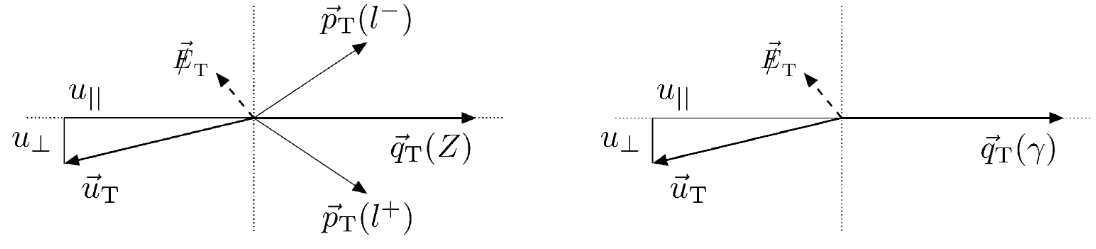
\includegraphics[width=0.95\textwidth]{MET}
\caption{ Z boson (left) and photon (right) kinematics with the vector of all the visible objects (denoted by u) and a resulting MET.}
\label{fig:MET}
\end{figure}


%following the twiki:
%\begin{center}
%\texttt{https://twiki.cern.ch/twiki/bin/viewauth/CMS/MissingETRun2Corrections}
%\end{center}
%On top, a set of filters related to the instrumental effects is employed:
%\begin{center}
%\texttt{https://twiki.cern.ch/twiki/bin/view/CMS/MissingETOptionalFiltersRun2}
%\end{center}
